\section{Data}
The frozen prepared dataset contains 57 participants: 19 dyslexia-labeled and 38
typical/control readers. The prepared tables contain 335,203 word-level rows, 1,986
sentence-level rows, and 57 participant-level rows. Table~\ref{tab:dataset-summary}
summarizes the dataset, and Table~\ref{tab:feature-label-release} summarizes the frozen
feature and label releases.

The analysis uses Feature Release v1 and Label Release v1.1. Quality labels record LM
missingness, parser status, and label availability. The parser status is
\texttt{surface\_heuristic\_fallback}, so no parser-syntax claim is made. Segmentation
labels are deterministic orthographic boundary-opacity proxies, not pronunciation-aware
labels. Text assignment is not randomized; this motivates the DFM exposure-only and
text-exposure sensitivity checks. All predictive validation is participant-grouped, with
leave-one-participant-out as the primary split policy.


\begin{table}[t]
\centering
\small
\caption{Dataset summary for the frozen Label Release v1.1 prepared tables.}
\label{tab:dataset-summary}
\begin{tabular}{lll}
\toprule
item & value & note \\
\midrule
participants\_total & 57 & prepared participants \\
dyslexia\_labeled & 19 & operational label \\
typical\_control & 38 & comparison group \\
word\_rows & 335203 & prepared word-level rows \\
sentence\_rows & 1986 & prepared sentence rows \\
\bottomrule
\end{tabular}
\end{table}

\begin{table}[t]
\centering
\small
\caption{Feature and label release provenance summary.}
\label{tab:feature-label-release}
\begin{tabular}{lll}
\toprule
item & value & note \\
\midrule
feature\_release\_dir & /home/haizhe/copco/results/feature\_release\_v1\_20260505\_2155 &  \\
status & complete &  \\
dfm\_model & danish-foundation-models/dfm-decoder-open-v0-7b-pt & primary LM \\
gemma\_status & pending & gated access \\
parser\_status & surface\_heuristic\_fallback & no syntax claims \\
\bottomrule
\end{tabular}
\end{table}

\begin{figure}[t]
\centering
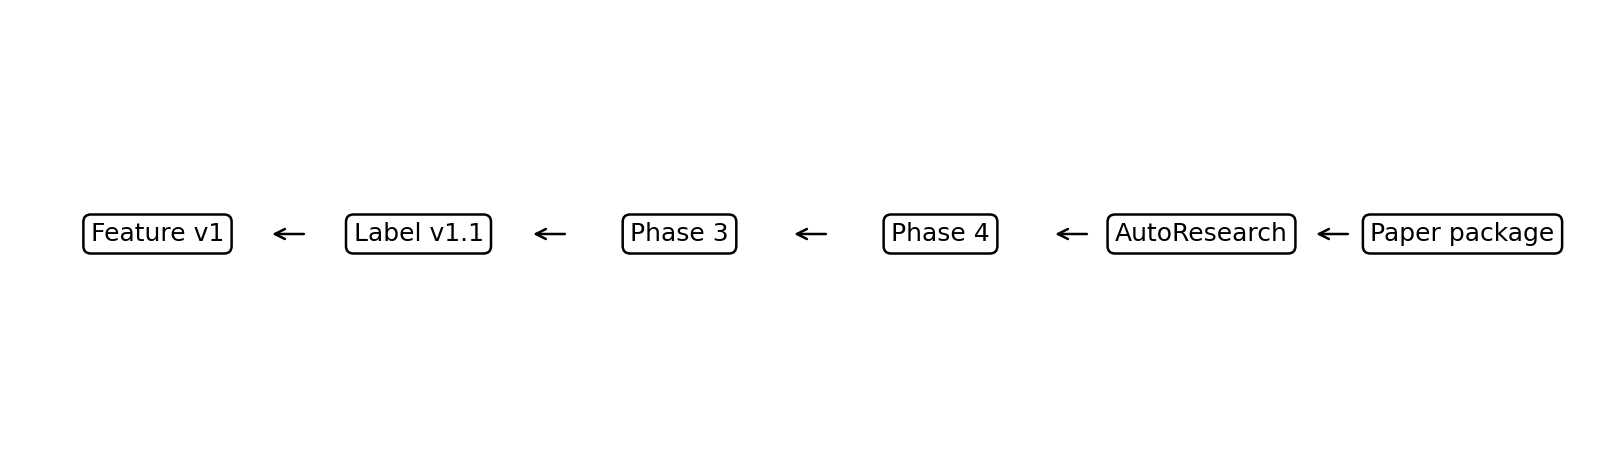
\includegraphics[width=0.92\linewidth]{figures/pipeline_overview.png}
\caption{End-to-end frozen analysis and submission package flow.}
\label{fig:pipeline-overview}
\end{figure}
